%!TEX root = ../thesis.tex

\section{背景}
近年,人手不足を背景にサービスロボットの需要が高まり,オフィスロボットの開発も様々な企業
や研究室で活発に行われている.代表的なロボットとして,PALロボティクス社が開発しているTIAGoとトヨタ自動車が開発しているHSRを示す.しかし,多くのオフィスロボットは設計データが公開されていない
ため,利用者による改良や新規開発が困難であり,研究開発への参入障壁となっている.一方,設計データを公開しているロボットは存在するものの,それらは主に情報共有を目的としており,必ずしもユーザーが容易に自作できる設計思想に基づいて開発されているわけではない.このため,研究開発用途に適した,容易に利用・改変可能なオープンプラットフォームなオフィスロボットは依然として不足しているのが現状である.

オープンプラットフォームハードウェアの成功事例として,i-Cartシリーズが挙げられる.自律
移動ロボットである i-Cart mini と i-Cart middle は,設計データ,部品リスト,組み立て図
が公開されており,誰もが容易に複製・改良できる.実際に,i-Cartをベースとした様々なロボットが開発されおり,自律移動ロボット開発の活性化に大きく貢献している.

オープンプラットフォームオフィスロボット開発の第一段階として,本研究ではロボットアームの
開発に取り組む.オフィス環境で活動するロボットは,人間と共同の空間での作業となるため人間に危害が及ぶ可能性を持っている.文献[1]では,ソフトウェア的にその問題解決に取り組んでいるが,本研究ではアクチュエータにQDDモータを使用し,ハードウェア的解決を目指す.
\begin{figure}[h]
  \centering
  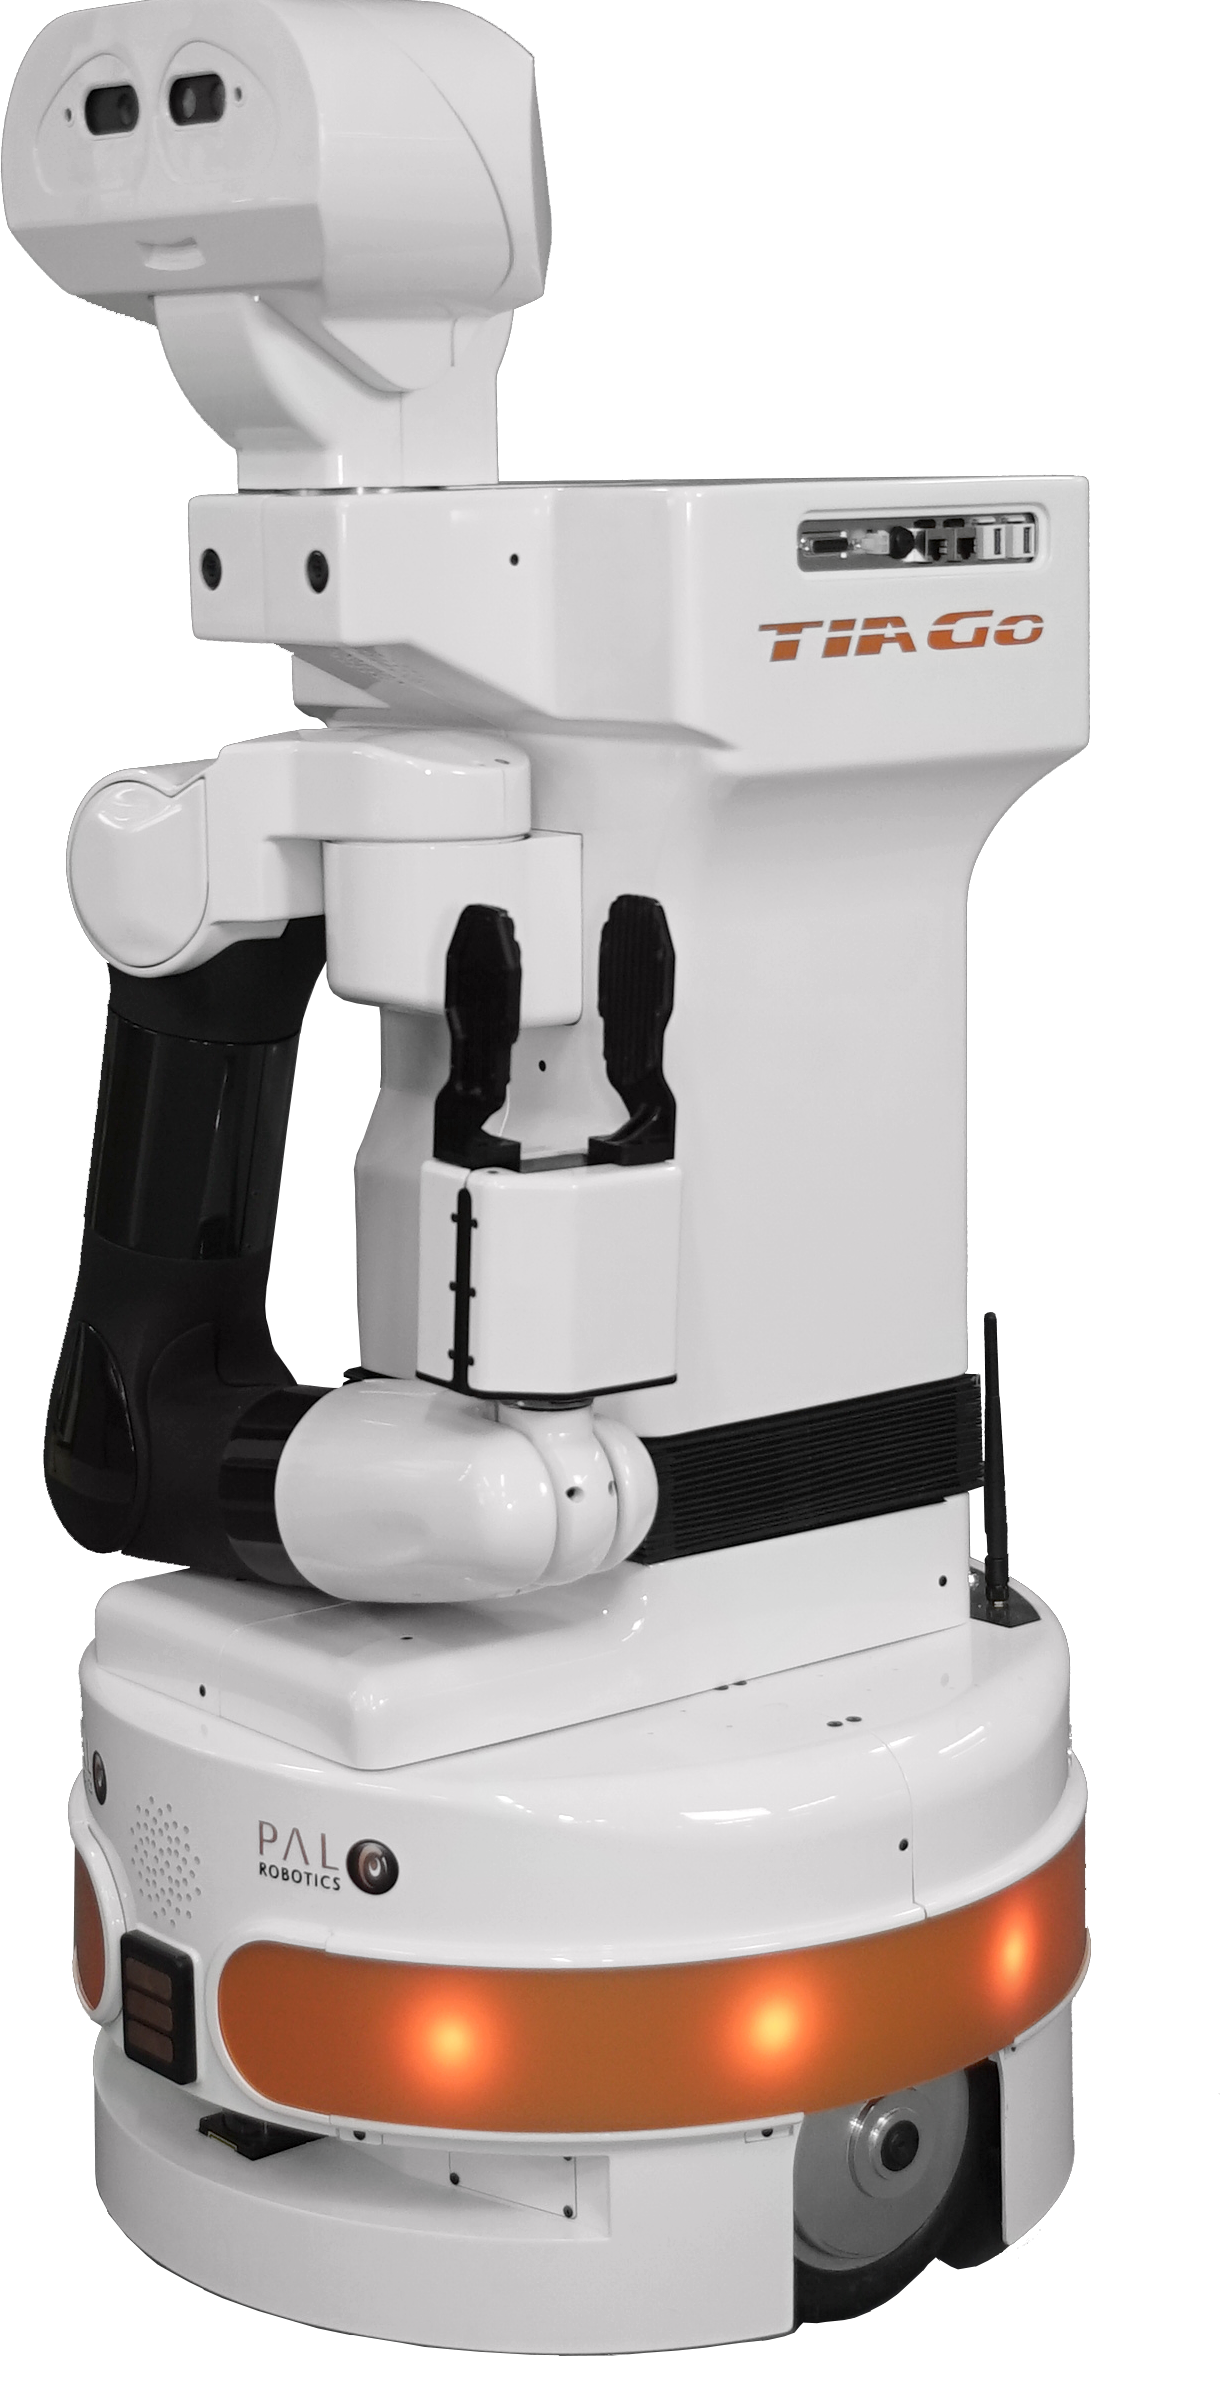
\includegraphics[width=25mm]{images/png/TIAGo.png}
  \caption{TIAGo from PAL-Robotics}
  \label{fig_TIAGo}
\end{figure}
\begin{figure}[h]
  \centering
  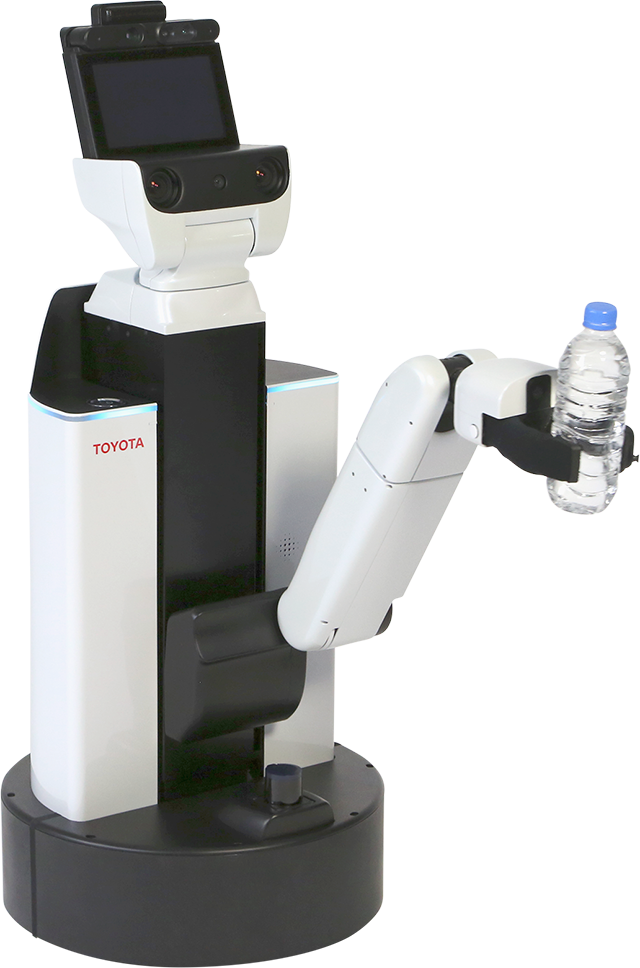
\includegraphics[width=25mm]{images/png/HSR.png}
  \caption{HSR from TOYOTA}
  \label{fig_HSR}
\end{figure}

\section{ロボットアーム調査とQDDモータ採用の動機}
既存のオフィスロボットのアームを調査した結果,4台のロボットアームに使用されているアクチュエータが判明した.Reachy,sobit pro,Mobile ALOHA,らのロボットアームはROBOTIS社のDynamixel(XM-430,XM-540,MX-106Tなど)を採用している.また,本研究室OBが過去に開発したオフィスロボットのアームには近藤科学のB3Mサーボモータ(B3M-SC-1040-A,B3M-SC-1170-A)を採用している.これらのサーボモータは多くのロボットに搭載されているもので,小型かつ高トルクなモータである.しかし,高減速比のためロボットアームの関節はバックドライバビリティが低くなってしまう.バックドライバビリティとは,機械工学事典にて,「アクチュエータや動力伝達機構において,出力節に適当な力を加えたときに,その節が可動し,かつそれが入力節側に伝わる性質.ダイレクトドライブモータや低減速比の平歯車を用いた駆動系などにこのような性質がみられる.」(引用:機械工学事典)と説明されている.つまり,通電時,関節が外力に対してどの程度柔軟に駆動するかというものだが,調査したロボットアームに搭載されているアクチュエータは高減速比のために外力に対して関節がほとんど動くことはない.衝突時に人間だけでなくロボットも守ることができる関節を実現するため,QDDモータを採用した.使用するQDDモータ(Steadywin GIM8108-8)と調査したサーボモータの比較を表に示す.DynamixelとB3Mの減速比に比べ,QDDモータの減速比が非常に小さいことがわかる.さらに,QDDモータは許容ラジアル荷重,許容アキシアル荷重が高いため,モータとリンクを部品でつなぐシンプルな構成のロボットアームの実現が可能であり,オープンプラットフォームとして好ましい.
\begin{table}[]
  \begin{tabular}{lccc}
  \hline
            & \begin{tabular}[c]{@{}c@{}}Dynamixel \\ MX-106T\end{tabular} & \begin{tabular}[c]{@{}c@{}}KONDO\\ B3M-CS-1170-A\end{tabular} & \begin{tabular}[c]{@{}c@{}}Steadywin\\ GIM8108-8\end{tabular} \\ \hline
  ストールトルク   & 8.0                                                          & 7.6                                                           & 22                                                            \\
  無負荷回転数    & 41                                                           & 46                                                            & 110                                                           \\
  減速比       & 225 : 1                                                      & 362.88 : 1                                                    & 8 : 1                                                         \\
  重量        & 153                                                          & 105                                                           & 396                                                           \\
  許容ラジアル荷重  & 40N                                                          & -                                                             & 900                                                           \\
  許容アキシアル荷重 & 20N                                                          & -                                                             & 800                                                           \\ \hline
  \end{tabular}
\end{table}
  
\section{関連研究}
\subsection{QDDモータを用いたロボットアーム}
近年,QDD(Quasi-Direct Drive)アクチュエータを用いたロボットアームの研究が注目を集めている.QDDアクチュエータは,高減速比ギアを用いることなくモータを直接,あるいは低減速比のギアを介して関節に接続する方式であり,バックドライバビリティと高帯域幅制御といった利点を持つ.Zhao ら[26]は,5自由度の軽量QDDロボットアームを提案している.この研究では,モバイルロボットへの搭載を想定し,軽量化,安全性,制御性能の向上を設計目標としている.彼らは,アームの軽量化のために,自由度を5に削減し,一部の関節にリモートアクチュエーション機構を採用している.また,リンク形状のトポロジー最適化や,高強度アルミニウム合金,樹脂3Dプリント部品の利用により,軽量化と構造的強度を両立させている.提示された論文では,ピックアンドプレースタスクを想定したシミュレーションと,実機によるコンプライアンス制御実験を行い,QDDアームの実現可能性を示している.

しかし,この研究ではオープンプラットフォーム化については考慮されておらず,具体的な作業タスクも設定されていない.
\begin{figure}
  \centering
  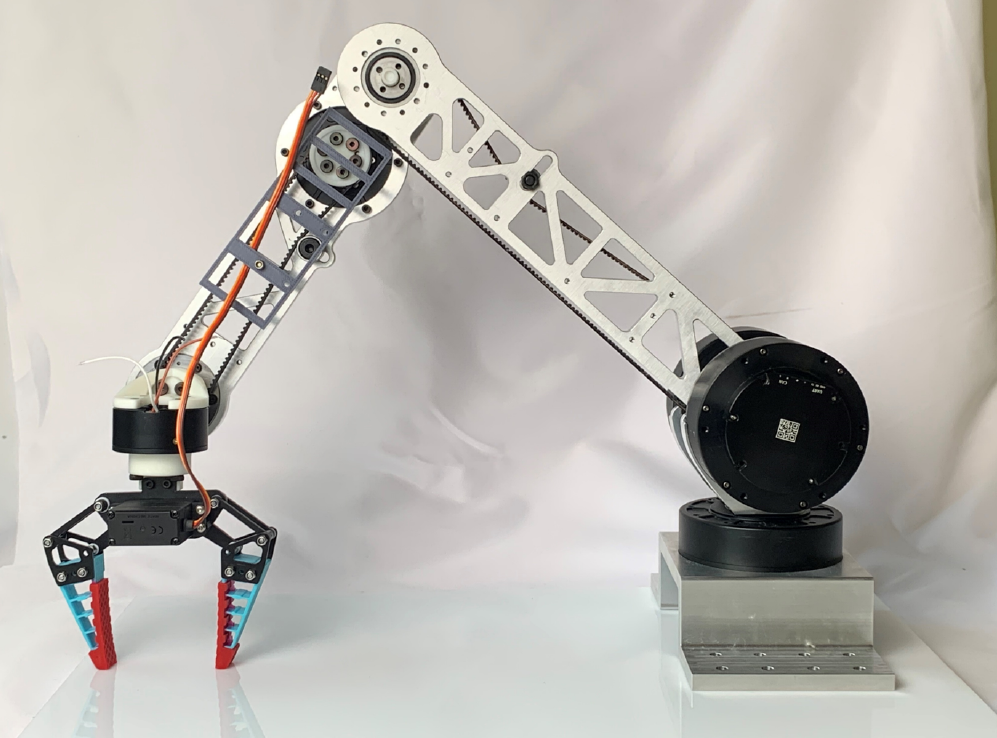
\includegraphics[width=10cm]{images/qddarm.png}
  \caption{The proposed 5-DOF articulated quasi-direct drive (QDD) robot arm,
  together with a commercial 1-DOF soft gripper.}
  \label{fig_qddarm}
\end{figure}

\section{目的}
 QDDモータを使用したロボットはいくつかあるが,ロボットアームに関しては不足している.また,オープンプラットフォームとなっているものもない.本研究は,オープンプラットフォームオフィスロボット開発の第一段階として,QDDモータを使用したロボットアームの設計と製作をすることを目的とする.
\section{本論文の構成}
 第1章は,研究背景や目的について述べ,本研究と関連する先行研究や文献について調査して,研究の位置づけを明らかにした.第2章では,対象とする作業の決定と要求仕様について述べる.第3章ではロボットアームの設計について述べる.第4章ではロボットアームの製作について述べる.第5章は結論として,まとめと今後の展望について述べる.

\newpage
